\documentclass{article}
% --- watermark (auto-inserted) ---
\usepackage{xcolor}
\usepackage{xfp}% \fpeval; in the kernel since 2022, harmless on older LaTeX
\usepackage{draftwatermark}
\newlength{\watermarkTextWidth}
\AddToHook{begindocument/end}{%
  \SetWatermarkText{\normalfont Generated by The Agentic Scientist}%
  \SetWatermarkFontSize{10pt}%
  \SetWatermarkLightness{0.85}%
  \settowidth{\watermarkTextWidth}{\normalfont\fontsize{10pt}{12pt}\selectfont Generated by The Agentic Scientist}%
  \edef\watermarkScale{\fpeval{0.8 * sqrt(\paperwidth**2 + \paperheight**2) / \watermarkTextWidth}}%
  \edef\watermarkAngle{\fpeval{atand(\paperheight/\paperwidth)}}%
  \SetWatermarkScale{\watermarkScale}%
  \SetWatermarkAngle{\watermarkAngle}%
}
% --- end watermark ---

\usepackage{paper,times}
\usepackage{amsmath,amssymb,graphicx,booktabs,subcaption,longtable}
\usepackage{hyperref,url}
\title{Fixed-Game SHAP Reliability:\\Structure, Budgets, and Reference Limits}
\author{}
\newcommand{\norm}[1]{\left\lVert #1\right\rVert_1}
\begin{document}
\maketitle

\begin{abstract}
A feature attribution can be repeatable without accurately computing its intended explanation, and accurate without justifying a decision. We isolate the computational question for frozen tabular classifiers: agreement with a fixed empirical, probability-scale Shapley game under finite coalition caps. We compare library Kernel SHAP, averaging two split-cap estimates, and structure-aware computation using forest leaf constraints and logistic integration. German Credit and an explicitly adapted ACS income task provide logistic and forest conditions with different reference quality. Across the retained final evaluation, structure-aware outputs have mean normalized reference agreement of 0.99756 and identical observed attribution vectors across repeated calls; their top-three sets agree with every reference. However, German references are approximate, and the structure-aware methods access model parameters rather than spending the same prediction-only budget. Split-cap averaging is particularly weak at the smallest German cap. These results support a narrow computational-reliability claim for the evaluated fixed games, not equal-time superiority, robustness to background changes, or reliable reasons for high-stakes decisions.
% @evidence[[paper_data.json#/final_evaluation/metrics/reference_fidelity]]
% @evidence[[analysis_summary.json#/max_repeat_vector_difference]]
% @evidence[[paper_data.json#/final_evaluation/evaluation_evidence/episodes]]
\end{abstract}

\section{Introduction}
Feature attributions are often presented as a compact rationale for an individual prediction. The SHAP framework assigns additive feature contributions using a Shapley-value construction \citep{Lundberg2017,Shapley1953}. Computing these contributions can require approximation, so an explanation obtained under a practical budget should be assessed as a numerical result, not accepted merely because the attribution interface returns a vector. This matters particularly when a small set of highly ranked features becomes the public-facing account of a credit or income prediction.

There are several distinct reliability questions. Does repeating the same calculation change the answer? Does the returned vector approximate the intended Shapley values? Is the underlying explanation game appropriate for the application? Does that game provide a justified reason for acting on the prediction? The first two are computational questions; they do not settle the latter two. Explanation disagreement across methods \citep{Krishna2022}, dependence on background data \citep{Yuan2022}, and the distinction between observational and interventional games \citep{Chen2020} make this separation essential.

We study a deliberately restricted setting: a frozen classifier, fixed query, fixed finite background, and a probability output. The central question is whether one returned attribution vector is dependable as a computation of that \emph{particular} game. Our hypothesis is that exploiting an exposed classifier's structure can remove substantial sampling error, but that repeatability alone remains insufficient evidence of attribution accuracy. The comparison is between computational access regimes, not just interchangeable random seeds: prediction-only estimators sample hybrid inputs, whereas the structure-aware implementation also uses tree arrays or logistic coefficients.

The study combines a held-out evaluation with matched development comparisons. The former supplies the principal measurements; the latter helps localize changes to the corresponding model family without presenting development selection as independent confirmation. Across the final German Credit and ACS conditions, observed repeated-call vectors are identical and normalized reference agreement is high. Crucially, exhaustive ACS references and approximate German references allow different strengths of interpretation. We retain this asymmetry rather than reporting every comparison as distance to ground truth.
% @evidence[[paper_data.json#/final_evaluation/evaluation_evidence/episodes]]

Our contributions are: (i) a fixed-game protocol that separately measures reference distance, top-feature membership, sign agreement, repeat consistency, and endpoint conservation; (ii) a concrete, inspectable comparison of sampled estimates with forest leaf-game and probability-scale logistic computations; and (iii) evidence about the limits of those measurements, including split-budget failure, approximate-reference disagreement, and unequal computational access. We do not claim a new general theory of explanation validity or a new invention of exact tree attribution. Figure~\ref{fig:overview} summarizes the evidence structure.

\begin{figure}[t]
\centering

\includegraphics[width=\textwidth]{figures/fixed_game_overview.png}
\caption{Computational reliability for a fixed explanation game. Sampled and structure-aware calculations target the same finite-background probability game. Repeat consistency and reference agreement answer different questions; neither establishes deployment validity.}
\label{fig:overview}
\end{figure}

\section{Related Work}
\paragraph{Attribution targets and computation.}
Shapley values originate in cooperative games \citep{Shapley1953}; SHAP connects this allocation principle to additive prediction explanations \citep{Lundberg2017}. Multilinear game extensions \citep{Owen1972} motivate integrating expected marginal contributions over inclusion probabilities. Sampling-based Shapley calculation \citep{Castro2009} and leverage-score sampling \citep{Musco2024} address computational cost without requiring tree-specific structure. Exact tree attribution is established prior work \citep{Lundberg2018}. Our contribution is the bounded empirical comparison and its interpretive limits, not priority for exact forest explanations. Leverage SHAP and a separate TreeSHAP implementation were not evaluated here.

\paragraph{Different meanings of stability.}
Practitioner-facing disagreement between explanation methods \citep{Krishna2022} differs from repeating a computation with the game fixed. Background-size effects in deep models \citep{Yuan2022} also change a source of variation that we hold constant. Interventional and observational expectations can answer different questions \citep{Chen2020}; accurate computation does not choose between them. Predictive multiplicity \citep{Marx2020} concerns competing trained models, whereas our primary repeat comparison freezes each fitted model. Feature-selection stability \citep{Nogueira2018} and rank-biased overlap \citep{Webber2010} provide context for comparing feature sets and rankings. Our reported top-three intersection is a simple membership measure, not either of those specialized statistics.

\paragraph{Uncertainty and scope.}
Bounds for independent bounded observations \citep{Hoeffding1963} and variance-sensitive empirical bounds \citep{Maurer2009} motivate internal safeguards in the sampled fallback. Their presence does not establish observed acceptance coverage. Bootstrap resampling \citep{Efron1979} supports conditional uncertainty over query instances, not an extrapolation over new populations. ACS-based tasks \citep{Ding2021} provide a public income setting; German Credit supplies a smaller credit setting \citep{GermanCredit}. Logistic regression \citep{Hosmer2013} and random forests \citep{Breiman2001} expose structures useful for this computational comparison. Tabular neural architectures \citep{Gorishniy2021} lie outside its measured model coverage.

\section{Method}
\subsection{Fixed-Game Target and Reliability Criteria}
Let $f:\mathbb{R}^d\rightarrow[0,1]$ be a frozen classifier's positive-class probability, $x$ a query, and $Z=(z_1,\ldots,z_B)$ a fixed background. A coalition $S\subseteq D=\{1,\ldots,d\}$ selects query coordinates and replaces all others with coordinates from one background row:
\begin{align}
 v_x(S)&=\frac{1}{B}\sum_{b=1}^B f(x_S,z_{b,D\setminus S}), \\
 \phi_j&=\sum_{S\subseteq D\setminus\{j\}}\frac{|S|!\,(d-|S|-1)!}{d!}
       \big[v_x(S\cup\{j\})-v_x(S)\big]. \label{eq:shapley}
\end{align}
This is an empirical replacement game, not a conditional-distribution estimator. Each supplied scalar-encoded original feature is a player. The probability scale and background remain identical across compared computations. In particular, logistic coefficients on the log-odds scale are not substituted for probability-scale attributions.
% @evidence[[source_evidence/selected/reliability.py#L11-L64]]
% @evidence[[source_evidence/evaluation/evaluate_final.py#L757-L796]]

For an estimate $\widehat\phi$ and recorded reference $\phi^{\rm ref}$, we use normalized L1 reference agreement
\begin{equation}
 A(\widehat\phi,\phi^{\rm ref})=
 \left(1+\frac{\norm{\widehat\phi-\phi^{\rm ref}}}
 {\max(\norm{\phi^{\rm ref}},10^{-3})}\right)^{-1}. \label{eq:agreement}
\end{equation}
The floor prevents division by a near-zero reference norm; the score is not a probability of explanation validity. Let $T(a)$ be the indices of the three largest $|a_j|$, with original coordinate order resolving ties. Reference top-three overlap is $|T(\widehat\phi)\cap T(\phi^{\rm ref})|/\min(3,d)$. Sign agreement is the fraction of coordinates with equal signs, treating magnitudes at most $10^{-8}$ as zero. We also report endpoint residual
\begin{equation}
 E=\min\!\left(1,\frac{|\sum_j\widehat\phi_j-[f(x)-v_x(\varnothing)]|}
 {\max(|f(x)-v_x(\varnothing)|,10^{-3})}\right).
\end{equation}
For each pair of repeated calls, we compute the same top-three and sign agreements between their outputs rather than against a reference. These pairwise summaries are kept separate from reference agreement throughout the paper. Endpoint conservation is a consistency check, not proof of correct feature allocation.
% @evidence[[source_evidence/evaluation/evaluate_final.py#L1014-L1030]]

\subsection{Compared Computations}
\paragraph{Prediction-only baselines.}
The library baseline uses \texttt{shap.KernelExplainer} with the identity link, no L1 selection penalty, and the requested coalition cap $C$. Its split-cap comparator averages independent estimates using $\lfloor C/2\rfloor$ samples each. Both use the same serialized probability predictor, background, and queries as the structure-aware implementation. This comparator evaluates budget splitting, not the effect of doubling total resources. Endpoints, background expansion, and setup costs mean a coalition cap is not a literal wall-time or total prediction-row equality.
% @evidence[[source_evidence/evaluation/evaluate_final.py#L757-L772]]
% @evidence[[source_evidence/evaluation/evaluate_final.py#L848-L871]]

\paragraph{Forest leaf-game computation.}
For every tree, the implementation intersects all splits on a feature along a root-to-leaf path. With query $x$ and background row $z_b$ fixed, a feature can satisfy the leaf constraint only when included, only when excluded, in both states, or in neither. A neither-state feature makes that leaf's game identically zero. Otherwise write $P$ for required inclusions and $Q$ for required exclusions, with sizes $p,q$; both-state features are dummy players. The leaf indicator is
\begin{equation}
 g(S)=\mathbf{1}\{P\subseteq S,\;Q\cap S=\varnothing\}.
\end{equation}
Integrating the inclusion-probability marginal gives contribution coefficients
\begin{equation}
 \phi_j(g)=\begin{cases}
   [p\binom{p+q}{p}]^{-1},&j\in P,\\
   -[q\binom{p+q}{p}]^{-1},&j\in Q,\\
   0,&j\notin P\cup Q.
 \end{cases} \label{eq:leaf}
\end{equation}
Multiplying by leaf probabilities and averaging over trees and background rows exploits Shapley linearity. This avoids sampled coalition predictions for the forest branch. The implementation respects repeated-feature splits and the supplied predictor's float32 input and float64 threshold semantics; exactness refers to this finite, serialized game, up to floating-point arithmetic.
% @evidence[[source_evidence/selected/forest.py#L11-L81]]
% @evidence[[source_evidence/evaluation/evaluate_final.py#L720-L755]]

\paragraph{Probability-scale logistic integration.}
For one background row define $a=\beta_0+\beta^\top z_b$ and $u_j=\beta_j(x_j-z_{bj})$. The coalition probability is $\sigma(a+\sum_{j\in S}u_j)$. The implemented sigmoid identity and inclusion integral yield
\begin{align}
 \sigma(s)&=\tfrac12+\int_0^\infty\frac{\sin(\omega s)}{\sinh(\pi\omega)}\,d\omega,\\
 \phi_j^{(b)}&=\int_0^\infty\!\frac{\operatorname{Im}\!\left[e^{i\omega a}(e^{i\omega u_j}-1)
 \int_0^1\prod_{k\ne j}(1-t+t e^{i\omega u_k})\,dt\right]}
 {\sinh(\pi\omega)}\,d\omega. \label{eq:logistic}
\end{align}
The inner polynomial has degree at most $d-1$, so $\lceil d/2\rceil$ Gauss--Legendre nodes integrate it exactly in exact arithmetic. Prefix/suffix products avoid division by possibly zero factors. The outer frequency integral is numerical, not an exact logistic SHAP solver.
% @evidence[[source_evidence/selected/logistic_fourier.py#L12-L40]]
% @evidence[[source_evidence/selected/logistic_fourier.py#L97-L140]]

The implementation truncates frequencies at 8, uses eight-node quadrature panels, and refines up to 2048 frequency nodes. It requires two consecutive mesh agreements and an endpoint residual within $10^{-8}$, with an analytic tail tolerance of $10^{-10}$. Mesh agreement does not bound every coordinate's discretization error. If any background row fails numerical checks, the whole logistic integration is rejected and the sampled fallback is retained. All supplied background rows are averaged; these checks do not select a favorable subset.
% @evidence[[source_evidence/selected/logistic_fourier.py#L43-L94]]

\paragraph{Dispatch and sampled fallback.}
Forest structure is used directly. Other games are enumerated when the cap covers their nontrivial coalitions; otherwise logistic integration is considered. The fallback combines independent complete permutation paths with complement-paired kernel-distributed masks and an importance-corrected, endpoint-constrained regression. An internal signed top-feature separation test may select the path estimate instead. We have no recorded dispatch frequencies or test-acceptance coverage and make no empirical certification claim. The source ordering matters: high-cap exhaustive behavior must not be attributed to quadrature alone.
% @evidence[[source_evidence/selected/reliability.py#L163-L197]]

\subsection{Design Rationale and Component Comparisons}
The design removes sampling where model structure permits same-game algebra, rather than changing what absent features mean. Forest leaf constraints expose a finite conjunction game; logistic additivity in the logit allows a probability-scale transform. We therefore expect the largest benefits where prediction-only estimates are inaccurate under the supplied cap. Deterministic computation is not itself the hypothesis test: an incorrect deterministic vector would be perfectly repeatable.

Two matched development comparisons examine the forest component with the nonforest computation retained, and logistic integration with the forest component retained. Readable source differences support this limited interpretation. These are narrower comparisons than a claim that every observed configuration difference isolates a single mathematical choice: the components also change access to model structure and computational work. There is no factorial study of quadrature safeguards, background size, or permutation-test acceptance.
% @evidence[[source_evidence/sampled/reliability.py]]
% @evidence[[source_evidence/forest/reliability.py]]
% @evidence[[source_evidence/selected/reliability.py]]

\section{Experimental Setup}
\paragraph{Data and frozen models.}
The final evaluation uses German Credit and ACSIncome-2024-RELSHIPP, each with logistic regression and a random forest. German retains 300 training, 100 validation, and 100 explanation records with 20 feature groups. ACS retains 20000, 6667, and 6667 records with 10 groups. Only the first 16 explanation records and first 16 training rows are used as queries and background in each condition; these are fixed across repeated calls, not randomly redrawn per explanation. Thus the split sizes should not be mistaken for the number of explained individuals.
% @evidence[[paper_data.json#/final_evaluation/evaluation_evidence/episodes]]
% @evidence[[source_evidence/evaluation/evaluate_final.py#L687-L718]]
% @evidence[[source_evidence/evaluation/capture.py#L61-L155]]

German records are partitioned by normalized predictor content into disjoint development and final subsets. ACS uses California for development and New York for final evaluation, after excluding cross-state predictor-content overlaps. The final ACS task replaces the historical \texttt{RELP} field, absent from the retained release schema, with native \texttt{RELSHIPP}; it is not bit-identical to historical ACSIncome. Other predictors, the adult population filter, and the income threshold are retained in the acquisition code. These choices define the evaluated population, not a population-representative survey analysis.
% @evidence[[source_evidence/evaluation/data_provenance.json]]
% @evidence[[source_evidence/evaluation/capture.py#L87-L155]]

Categorical vocabularies are fitted on training data and encoded ordinally; numerical missing values use training medians. Training means and standard deviations standardize all supplied groups. No one-hot masking study is included. Logistic models use \texttt{lbfgs}, a 500-iteration cap and tolerance $10^{-7}$. Forests use 64 trees, maximum depth 6, and a single training thread. Model parameters and preprocessing remain frozen within a repeat comparison. Ordinal categories can impose artificial order; our results concern these fitted predictors, not optimal credit or income models.
% @evidence[[source_evidence/evaluation/evaluate_final.py#L687-L718]]
% @evidence[[source_evidence/evaluation/evaluate_final.py#L817-L848]]

\paragraph{Caps, seeds, and references.}
Final caps are 64, 256, and 1024. Each condition has six repeated structure-aware calls per cap for seeds 104729, 130363, and 155921. Each seed produces a fitted model/reference evaluation; queries and backgrounds are reused. ACS references enumerate all coalitions of the ten-feature game. German references average two independent library estimates, each with cap 4096. Their coordinatewise half-difference is retained as a reference-disagreement proxy, not a confidence interval or an error bound for their mean.
% @evidence[[paper_data.json#/final_evaluation/evaluation_evidence/episodes]]
% @evidence[[source_evidence/evaluation/evaluate_final.py#L848-L858]]
% @evidence[[source_evidence/evaluation/evaluate_final.py#L1314-L1320]]

\paragraph{Reporting and uncertainty.}
We average metrics over query instances within each condition, then over the recorded seeds with equal weights. Repeated calls on the same query are not independent individuals. The stored 95\% intervals resample the 16 query-level mean agreements using 1000 bootstrap resamples, after averaging caps and repeats within each fitted condition. They are neither pairwise-method confidence intervals nor uncertainty over retraining, background selection, or future deployment. Main plots show seed-level points and means, not invented standard errors. Library comparators have one recorded estimate per seed and cap; their within-model repeated-call consistency was not measured by this final protocol.
% @evidence[[source_evidence/evaluation/evaluate_final.py#L1154-L1159]]
% @evidence[[paper_data.json#/final_evaluation/evaluation_evidence/episodes]]

The completed final evaluation met its documented qualification checks. This establishes coverage and execution/control requirements, not semantic validity or a performance-based deployment threshold. No missing or failed empirical cell is used as evidence of inferiority. The full evaluation workload took 700.37 seconds of wall time, including references and comparators; candidate-only latency and total CPU-hours are unavailable. Development comparisons use two seeds, smaller query sets, and caps 64 and 256 and are reported separately.
% @evidence[[paper_data.json#/final_evaluation/status]]
% @evidence[[paper_data.json#/final_evaluation/outcome]]
% @evidence[[paper_data.json#/final_evaluation/metrics/wall_seconds]]
% @evidence[[paper_data.json#/all_programs]]

\section{Results}
\subsection{Main Fixed-Game Comparison}
Figure~\ref{fig:final} compares computations within each dataset/model condition. At cap 64, mean structure-aware agreement is 0.9966 for German logistic and 0.9937 for German forest, against 0.9347 and 0.8806 for the one-shot library baseline. On ACS, both structure-aware conditions round to 1.0000 against the exhaustive reference. The corresponding one-shot library means are 0.9577 and 0.9636. These comparisons support improved numerical agreement in the retained low-cap settings, not a claim about new people, backgrounds, or classifiers.
% @evidence[[analysis_summary.json#/final]]

\begin{figure}[t]
\centering
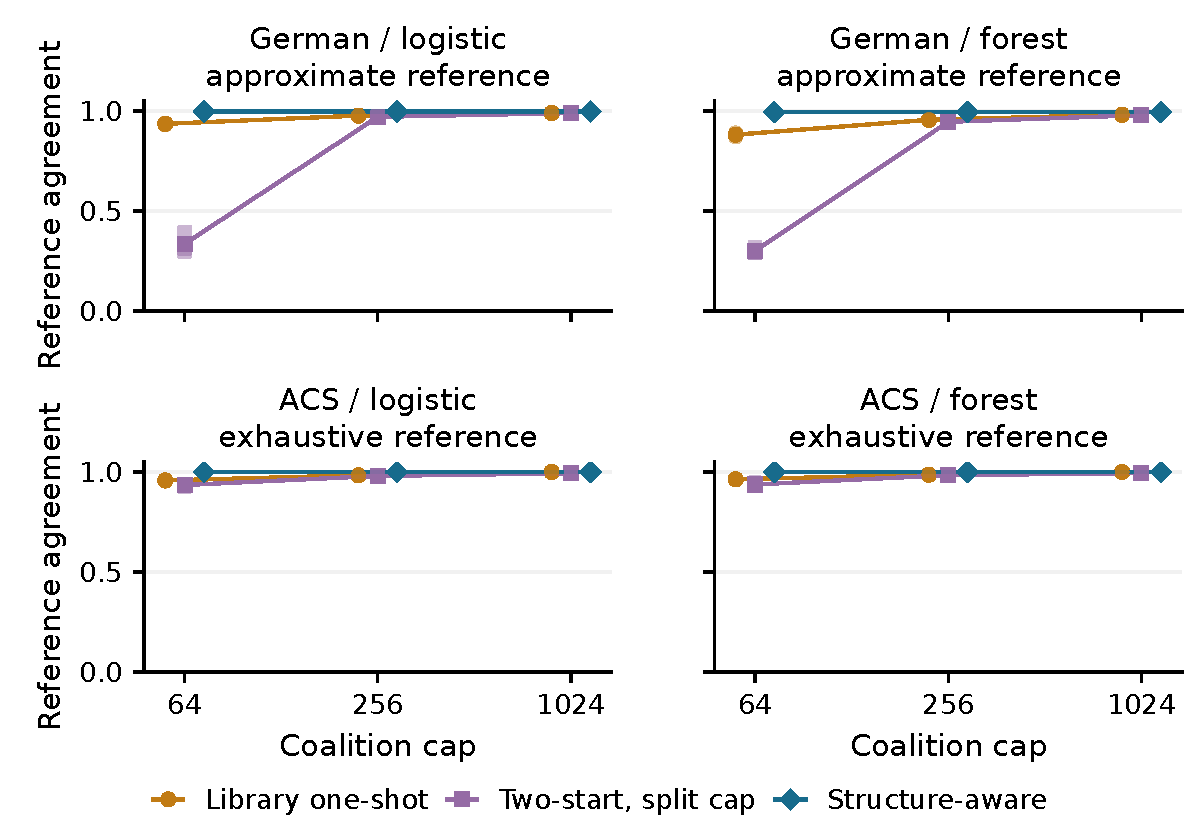
\includegraphics[width=\textwidth]{figures/final_reference_comparison.pdf}
\caption{Final reference agreement by dataset, classifier, and coalition cap. Dots show the three fitted-condition seeds; lines connect cap-wise means, not a temporal trajectory. German references average two high-cap estimates; ACS references are exhaustive. The common zero-to-one scale makes the severe split-cap German failure visible; Table~\ref{tab:main} resolves near-ceiling differences.}
\label{fig:final}
% @evidence[[paper_data.json#/final_evaluation/evaluation_evidence/episodes]]
\end{figure}

\begin{table}[t]
\centering
\caption{Final cap-64 mean reference agreement and structure-aware reference sign agreement, averaged over seeds. The top-three reference overlap is 1 throughout for the structure-aware computation. Values rounded to 1.0000 are not claims of exact real-arithmetic equality.}
\label{tab:main}
\small
\begin{tabular}{lrrrr}
\toprule
Condition & One-shot & Split cap & Structure & Signs\\
\midrule
% @evidence[[paper_data.json#/final_evaluation/evaluation_evidence/episodes]]
German / logistic & 0.9347 & 0.3341 & 0.9966 & 1.0000 \\
German / forest & 0.8806 & 0.2995 & 0.9937 & 0.9979 \\
ACS / logistic & 0.9577 & 0.9349 & 1.0000 & 1.0000 \\
ACS / forest & 0.9636 & 0.9378 & 1.0000 & 1.0000 \\
\bottomrule
\end{tabular}
% @evidence[[analysis_summary.json#/final]]
\end{table}

Increasing the library cap improves mean reference agreement in all four final conditions. At cap 1024, its German logistic and forest means reach 0.9889 and 0.9802, while both ACS means round to 1.0000. The implemented exhaustive dispatch can also apply at this ACS cap. The evidence therefore does not support saying that structure-aware computation is necessary for high agreement in every measured setting. Nor does an unchanged structure-aware curve establish budget efficiency: parameter access allows computations that are not charged as coalition predictions.
% @evidence[[analysis_summary.json#/final]]
% @evidence[[source_evidence/selected/reliability.py#L173-L184]]

The recorded aggregate normalized reference agreement is 0.9975639. We do not use the evaluator's mixed sign summary as if it were pure reference agreement: directly pooling the recorded reference-comparison cells gives sign agreement 0.9994792. Every structure-aware top-three set agrees with its reference, yet near-perfect membership and signs do not imply identical attribution magnitudes. Supplementary tables preserve the condition- and seed-level evidence instead of collapsing reference quality into a single success label.
% @evidence[[paper_data.json#/final_evaluation/metrics/reference_fidelity]]
% @evidence[[analysis_summary.json#/reference_sign_mean]]
% @evidence[[paper_data.json#/final_evaluation/evaluation_evidence/episodes]]

\subsection{Repeat Consistency Is Stronger Than Observed Reference Equality}
All retained structure-aware repeat-pair top-three and sign agreements equal 1. Inspecting the stored vectors also yields a maximum coordinate range across repeats of zero. This is consistent with deterministic dispatch in these conditions, but dispatch counts are not recorded. It does not show that an arbitrary fallback call will be deterministic or accurately attributed. There are only six calls per cap on a small fixed query set, and no population-level zero-failure guarantee follows.
% @evidence[[paper_data.json#/final_evaluation/evaluation_evidence/episodes]]
% @evidence[[analysis_summary.json#/max_repeat_vector_difference]]

German provides a useful separation: identical repeated outputs still differ from the approximate reference. The recorded query-bootstrap interval for German logistic at seed 104729 is $[0.99618,0.99709]$; the analogous forest interval is $[0.99292,0.99442]$. These intervals describe query heterogeneity conditional on the recorded reference, not uncertainty about the true Shapley vector. The mean absolute coordinate half-differences between German reference replicates are approximately $1.05\times10^{-4}$ for logistic and $1.20\times10^{-4}$ for forests. We cannot attribute all residual estimate-to-reference distance to either side from that proxy alone.
% @evidence[[paper_data.json#/final_evaluation/evaluation_evidence/episodes/0/solution/cases/0/observations/fidelity_instance_bootstrap_ci95]]
% @evidence[[paper_data.json#/final_evaluation/evaluation_evidence/episodes/0/solution/cases/1/observations/fidelity_instance_bootstrap_ci95]]
% @evidence[[analysis_summary.json#/reference_uncertainty]]

ACS has a stronger computational interpretation because its reference exhausts the specified finite game. Agreement there supports numerical fidelity to that game, without validating background choice or impossible hybrid records. The observed endpoint residual averages $1.28\times10^{-11}$; recorded control pass rate is 1, failed-call fraction is zero, and replay error is zero. These are narrow numerical and operational checks, not independent evidence that feature attributions are good reasons for decisions.
% @evidence[[paper_data.json#/final_evaluation/metrics/efficiency_error]]
% @evidence[[paper_data.json#/final_evaluation/metrics/control_pass_rate]]
% @evidence[[paper_data.json#/final_evaluation/metrics/failed_fraction]]
% @evidence[[paper_data.json#/final_evaluation/metrics/replay_error]]

\subsection{Budget Splitting and Component Sensitivity}
Averaging is not automatically helpful under a fixed total cap. At cap 64 the split-cap German logistic mean is 0.3341 and the forest mean is 0.2995, substantially below the one-shot means. By cap 256 those split-cap means recover to 0.9699 and 0.9448. The result establishes a failure of this particular low-cap split, not a general failure of averaging independent estimators. The retained diagnostics do not identify a unique numerical cause; reduced fit information is a plausible interpretation, not a measured mechanism.
% @evidence[[analysis_summary.json#/final]]

\begin{figure}[t]
\centering
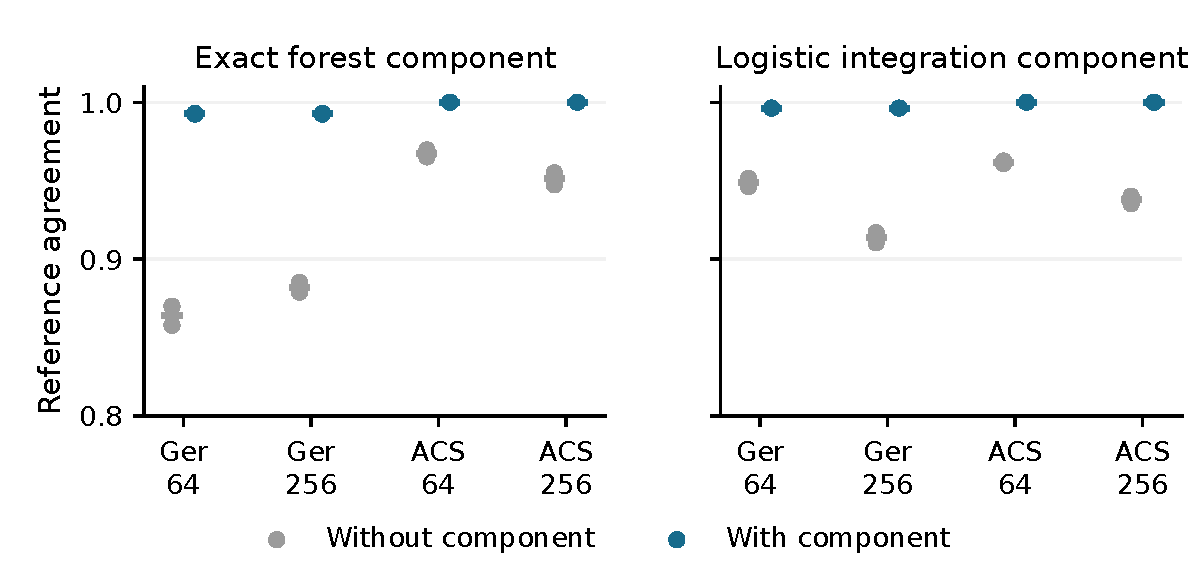
\includegraphics[width=\textwidth]{figures/component_comparison.pdf}
\caption{Matched component comparisons on development data only. Left: forest computation with and without the exact leaf-game component. Right: logistic computation with and without integration. Each category shows the two recorded seed values and a mean tick; the vertical axis is restricted to $[0.8,1]$. Ger/ACS denote dataset and labels underneath give coalition caps. The unchanged model family is retained in each comparison; structural access and work still differ.}
\label{fig:components}
% @evidence[[paper_data.json#/all_programs]]
\end{figure}

Development comparisons in Figure~\ref{fig:components} support family-localized changes. At cap 64, German forest reference agreement changes from 0.858--0.870 without the leaf-game component to 0.9924--0.9929 with it. German logistic changes from 0.946--0.951 without integration to approximately 0.9963 with integration. In both ACS comparisons, the structure-aware outputs agree with exhaustive references to the displayed precision. These are matched configuration comparisons, not evidence that an untested safeguard or formula alone caused every gain.
% @evidence[[analysis_summary.json#/development]]

The sampled development estimates also show nonmonotone cap behavior: ACS forest mean agreement without its structure component falls from approximately 0.9674 at cap 64 to 0.9512 at cap 256. German logistic without integration similarly falls from about 0.9488 to 0.9137. This concerns the custom sampled fallback, not the final library curve. More sampled coalitions need not improve an individual finite estimate, and the recorded comparisons do not isolate whether sampling mix, fit conditioning, or another interaction explains the pattern. No missing ablation is treated as a measured failure.
% @evidence[[analysis_summary.json#/development]]

\section{Discussion and Limitations}
\paragraph{What a single explanation supports.}
For these retained games, a single structure-aware output is empirically representative of its repeated-call outputs and closely matches the available reference. This is a statement about computation. A deployment policy still needs a tolerance on magnitude error, ranking errors, and sign errors that reflects its use case. We did not evaluate such a policy, elicited human requirements, or a threshold determining when a vector is sufficiently reliable to justify a decision. In particular, high mean agreement can hide rare query-specific behavior and the normalization in Equation~\ref{eq:agreement} does not directly encode decision harm.

\paragraph{Reference and dependence limits.}
The German reference's own approximation prevents assigning all remaining discrepancy to the tested method. Exhaustive ACS attribution removes that specific ambiguity, not the choice of game. The small fixed background, ordinal feature representation, and replacement of missing features can create unrealistic hybrids. There is no conditional-game, background-shift, refitting-stability, adversarial, or user study. Fixed queries are reused across seeds, so pooled cells and the many repeat pairs do not create a large independent sample. Bootstrap intervals do not account for shared reference bias.

\paragraph{Access, selection, and external validity.}
Structure-aware computation uses more information than a prediction-only service may expose. We lack candidate-only timing, branch counts, and equal-time comparisons. It is therefore inappropriate to translate the cap-wise agreement advantage into an unrestricted speed or cost advantage. Development selection introduces adaptivity; the held-out evaluation narrows but does not eliminate all selection concerns. The source protocol supplies only two tabular datasets and two model families, with few queries. Geographic separation for ACS is not a claim of cross-task generalization to medicine, other years, or neural models. Source inspection supports the released computational mechanisms, while unexecuted independent validation scripts are not counted as additional experimental evidence.

\paragraph{Scope of the contribution.}
The strongest supported finding is conditional: structural access can produce repeatable, reference-consistent computations of the chosen finite game under the supplied caps. This does not establish universal reliability of one-shot SHAP, superiority over unmeasured estimators, or validity of its use in high-risk decisions. The negative split-cap result and the unresolved German reference discrepancy are part of that finding, not exceptions to remove from the report.

\section{Conclusion}
Computational reliability of a feature attribution should distinguish repeating an answer from computing the intended answer. For the frozen German Credit and adapted ACS income models studied here, forest leaf-game attribution and probability-scale logistic integration yield identical observed repeated-call vectors and high agreement with their respective references. The library baseline approaches exhaustive ACS agreement at the largest cap, while dividing a small cap between two estimates can be substantially worse than one library call. Thus neither repeated execution nor averaging supplies a universal remedy.

The strength of the conclusion depends on what is held fixed and what is known. Exhaustive finite-game references support a sharper computational interpretation than approximate references. Structural access, fixed backgrounds, and a small reused query set prevent equal-time or broad deployment claims. A reliable numerical solution is one prerequisite for using an attribution, not evidence that the background, feature semantics, classifier, or downstream decision is justified. Future assessments need application-specific tolerances, broader query coverage, reference diagnostics, and matched cost accounting before making that stronger claim.

\clearpage
\bibliography{references}
\bibliographystyle{paper}
\clearpage
\appendix
\section{Supplementary Information}

\subsection{Fixed-Game Construction, Data Provenance, and Models}
The public acquisition and split implementation is included as
\texttt{source\_evidence/evaluation/capture.py}; data URLs, release digests, licenses, and the schema adapter are in \texttt{source\_evidence/evaluation/data\_provenance.json}. German Credit originates from UCI DOI 10.24432/C5NC77 under CC BY 4.0. ACS records originate from the 2024 one-year California and New York PUMS releases. The folktables code is MIT-licensed; the Census materials are public government data with site terms archived by the original acquisition. No separate SPDX data license is inferred.
% @evidence[[source_evidence/evaluation/data_provenance.json]]

The acquisition hashes normalized raw predictor content before population filtering, splitting, or preprocessing. Numeric fields use canonical finite decimal strings, categorical fields use Unicode normalization and normalized whitespace, and missing values have a typed sentinel. Predictor hashes exclude identifiers and labels. German content groups are split between development and final data, then deterministically partitioned into training, validation, and explanation subsets. All California/New York predictor-content overlaps are removed before ACS content groups are selected. Such exclusion changes population composition and does not substitute for population weighting.
% @evidence[[source_evidence/evaluation/capture.py#L41-L155]]

ACS uses \texttt{AGEP, COW, SCHL, MAR, OCCP, POBP, RELSHIPP, WKHP, SEX, RAC1P}. The acquisition retains the adult income population restriction and the binary \texttt{PINCP>50000} target. Native \texttt{RELSHIPP} is used without inventing a crosswalk to the absent \texttt{RELP}. German positive labels correspond to the original code 2. These target conventions matter when interpreting attribution signs; a positive value raises the serialized model's chosen positive-class probability, not an abstract notion of benefit.
% @evidence[[source_evidence/evaluation/capture.py#L72-L151]]

Training vocabularies map sorted categorical values to integer codes, with unseen values mapped to $-1$. Numeric imputation and all scaling statistics are training-fitted. The serialized predictor is checked against the fitted estimator on queries and background before explanation. This is a finite probe check, not proof of equivalent behavior on every hybrid input. Final validation accuracies are 0.67 for German logistic, 0.65--0.69 for German forests, approximately 0.7609 for ACS logistic and 0.7755--0.7773 for ACS forests. Logistic fits report convergence with 19 iterations on German and 13 on ACS. These diagnostics characterize the explained predictors; the attribution study does not establish predictive adequacy.
% @evidence[[source_evidence/evaluation/evaluate_final.py#L687-L718]]
% @evidence[[source_evidence/evaluation/evaluate_final.py#L838-L847]]
% @evidence[[paper_data.json#/final_evaluation/evaluation_evidence/episodes]]

\subsection{Structure-Aware Computation and Numerical Safeguards}
\paragraph{Leaf contributions.}
For a viable leaf, the expected indicator under independent feature inclusion with probability $t$ is $t^p(1-t)^q$. Including a required-positive feature changes this by $t^{p-1}(1-t)^q$, while including a required-negative feature changes it by $-t^p(1-t)^{q-1}$. Integrating each marginal from zero to one yields Equation~\ref{eq:leaf}. Features not constrained by that leaf contribute zero. A constant leaf contributes no feature attribution, though it contributes to the empty/full value. Repeated splits are intersected into lower-exclusive and upper-inclusive bounds; contradictory paths are removed. The exact finite-game claim depends on matching these traversal semantics.
% @evidence[[source_evidence/selected/forest.py#L11-L81]]

\paragraph{Frequency truncation is not discretization certification.}
In Equation~\ref{eq:logistic}, the phase difference has magnitude at most two and every inclusion factor has magnitude at most one. Thus the omitted tail beyond frequency $W$ is bounded coordinatewise by
\begin{equation}
 2\int_W^\infty\frac{d\omega}{\sinh(\pi\omega)}
 =-\frac{2}{\pi}\log\tanh\!\left(\frac{\pi W}{2}\right).
\end{equation}
This is the source implementation's frequency-tail bound. It does not bound mesh discretization error on the retained interval. The implementation uses agreement under refinement and endpoint conservation as additional numerical diagnostics, rejects nonfinite arithmetic or excessive phase ranges, and averages all background rows only after successful integration. Prefix/suffix products keep zero mixture factors well-defined. The wrapper catches floating-point overflow and invalid arithmetic and returns rejection without consuming the sampling generator.
% @evidence[[source_evidence/selected/logistic_fourier.py#L12-L140]]

\paragraph{Fallback safeguards.}
Independent permutation paths provide bounded marginal observations in $[-1,1]$. For $m$ complete paths, coordinate sample variance $s_j^2$, and $\alpha=0.05$, the implemented simultaneous radius is
\begin{equation}
 r_j=\sqrt{\frac{2s_j^2\log(4d/\alpha)}{m}}
       +\frac{14\log(4d/\alpha)}{3(m-1)}.
\end{equation}
It is used only when at least two complete paths exist. The path estimate is selected only when absolute-value intervals strictly separate selected from excluded features and the selected signs exclude zero. Otherwise regression is retained. Even if the underlying bound's conditions hold, this is not a guarantee conditional on selection and supplies no observed certification rate here. Permutation paths, not individual within-path marginals, are independent sampling units. Endpoint-constrained regression is not covered by that path-bound calculation.
% @evidence[[source_evidence/selected/reliability.py#L66-L161]]

\paragraph{Implementation evidence.}
Readable files in \texttt{source\_evidence/selected/} contain dispatch, integration, forest calculation, and the attribution-only response interface. The corresponding development snapshots are in \texttt{source\_evidence/sampled/} and \texttt{source\_evidence/forest/}. The release includes independent small-tree and logistic validation routines, but there is no recorded execution of those routines in the retained research evidence. They are not additional controls, replications, or measured ablations. Provenance hashes identify artifacts; the equations above are supported by the readable source, not merely by a prior audit verdict.
% @evidence[[source_evidence/selected/validate_forest.py]]
% @evidence[[source_evidence/selected/validate_logistic_fourier.py]]

Concrete source anchors are \path{source_evidence/selected/forest.py:11} for path intersections and leaf contributions,
\path{source_evidence/selected/logistic_fourier.py:12} for the numerical integrand and refinements,
and \path{source_evidence/selected/reliability.py:163} for dispatch. Metric definitions are in
\path{source_evidence/evaluation/evaluate_final.py:1014}.

\subsection{Episode-Level Reliability and Reference Uncertainty}
Table~\ref{tab:extended} lists every final non-replay condition and cap. Means within each row average the fixed query set and, for structure-aware outputs, repeated calls. No new evaluation is run to create this table. Table~\ref{tab:intervals} preserves the stored query-bootstrap intervals, averaged over caps and repeated calls as specified in the main text. They must not be read as uncertainty for the difference between two methods.
% @evidence[[paper_data.json#/final_evaluation/evaluation_evidence/episodes]]

\begin{longtable}{llrrrr}
\caption{Final seed/condition/cap reference agreement. Display precision can hide residual error near one.}\label{tab:extended}\\
\toprule Seed & Condition & Cap & One-shot & Split cap & Structure\\\midrule
\endfirsthead
\toprule Seed & Condition & Cap & One-shot & Split cap & Structure\\\midrule
\endhead
% @evidence[[paper_data.json#/final_evaluation/evaluation_evidence/episodes]]
104729 & German / logistic & 64 & 0.9292 & 0.3134 & 0.9967 \\
104729 & German / logistic & 256 & 0.9754 & 0.9713 & 0.9967 \\
104729 & German / logistic & 1024 & 0.9894 & 0.9893 & 0.9967 \\
104729 & German / forest & 64 & 0.8836 & 0.2904 & 0.9937 \\
104729 & German / forest & 256 & 0.9547 & 0.9454 & 0.9937 \\
104729 & German / forest & 1024 & 0.9806 & 0.9777 & 0.9937 \\
104729 & ACS / logistic & 64 & 0.9604 & 0.9363 & 1.0000 \\
104729 & ACS / logistic & 256 & 0.9834 & 0.9804 & 1.0000 \\
104729 & ACS / logistic & 1024 & 1.0000 & 0.9936 & 1.0000 \\
104729 & ACS / forest & 64 & 0.9604 & 0.9348 & 1.0000 \\
104729 & ACS / forest & 256 & 0.9853 & 0.9843 & 1.0000 \\
104729 & ACS / forest & 1024 & 1.0000 & 0.9942 & 1.0000 \\
130363 & German / logistic & 64 & 0.9361 & 0.3912 & 0.9966 \\
130363 & German / logistic & 256 & 0.9764 & 0.9670 & 0.9966 \\
130363 & German / logistic & 1024 & 0.9880 & 0.9889 & 0.9966 \\
130363 & German / forest & 64 & 0.8689 & 0.2905 & 0.9935 \\
130363 & German / forest & 256 & 0.9567 & 0.9421 & 0.9935 \\
130363 & German / forest & 1024 & 0.9787 & 0.9779 & 0.9935 \\
130363 & ACS / logistic & 64 & 0.9584 & 0.9397 & 1.0000 \\
130363 & ACS / logistic & 256 & 0.9834 & 0.9809 & 1.0000 \\
130363 & ACS / logistic & 1024 & 1.0000 & 0.9928 & 1.0000 \\
130363 & ACS / forest & 64 & 0.9666 & 0.9456 & 1.0000 \\
130363 & ACS / forest & 256 & 0.9877 & 0.9862 & 1.0000 \\
130363 & ACS / forest & 1024 & 1.0000 & 0.9940 & 1.0000 \\
155921 & German / logistic & 64 & 0.9388 & 0.2977 & 0.9964 \\
155921 & German / logistic & 256 & 0.9761 & 0.9712 & 0.9964 \\
155921 & German / logistic & 1024 & 0.9894 & 0.9871 & 0.9964 \\
155921 & German / forest & 64 & 0.8894 & 0.3178 & 0.9939 \\
155921 & German / forest & 256 & 0.9533 & 0.9470 & 0.9939 \\
155921 & German / forest & 1024 & 0.9813 & 0.9790 & 0.9939 \\
155921 & ACS / logistic & 64 & 0.9544 & 0.9288 & 1.0000 \\
155921 & ACS / logistic & 256 & 0.9838 & 0.9797 & 1.0000 \\
155921 & ACS / logistic & 1024 & 1.0000 & 0.9939 & 1.0000 \\
155921 & ACS / forest & 64 & 0.9639 & 0.9328 & 1.0000 \\
155921 & ACS / forest & 256 & 0.9860 & 0.9818 & 1.0000 \\
155921 & ACS / forest & 1024 & 1.0000 & 0.9945 & 1.0000 \\
\bottomrule
\end{longtable}

\begin{table}[t]
\centering
\caption{Stored 95\% instance-bootstrap intervals for structure-aware reference agreement, conditional on each fitted model and reference. ACS values rounding to one have residuals below the displayed resolution.}
\label{tab:intervals}
\small
\begin{tabular}{lll}
\toprule Seed & Condition & Interval\\\midrule
% @evidence[[paper_data.json#/final_evaluation/evaluation_evidence/episodes]]
104729 & German / logistic & [0.9961794823, 0.9970868158] \\
104729 & German / forest & [0.9929222303, 0.9944210303] \\
104729 & ACS / logistic & [1.0000000000, 1.0000000000] \\
104729 & ACS / forest & [1.0000000000, 1.0000000000] \\
130363 & German / logistic & [0.9960508216, 0.9970566319] \\
130363 & German / forest & [0.9924407908, 0.9945685087] \\
130363 & ACS / logistic & [1.0000000000, 1.0000000000] \\
130363 & ACS / forest & [1.0000000000, 1.0000000000] \\
155921 & German / logistic & [0.9959843487, 0.9968429357] \\
155921 & German / forest & [0.9928739317, 0.9947199151] \\
155921 & ACS / logistic & [1.0000000000, 1.0000000000] \\
155921 & ACS / forest & [1.0000000000, 1.0000000000] \\
\bottomrule
\end{tabular}
% @evidence[[paper_data.json#/final_evaluation/evaluation_evidence/episodes]]
\end{table}

\begin{figure}[t]
\centering
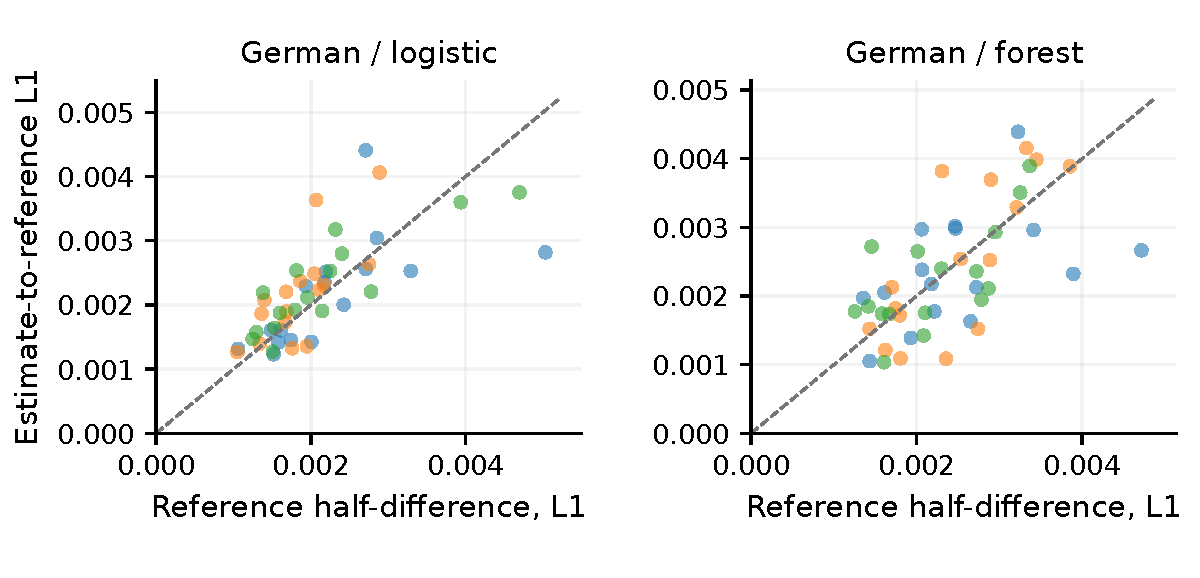
\includegraphics[width=\textwidth]{figures/reference_diagnostics.pdf}
\caption{German reference diagnostics. Each dot is a retained query/seed pair; color distinguishes seeds. The horizontal coordinate is the L1 norm of the two reference estimates' coordinatewise half-difference. The vertical coordinate is structure-aware distance to their mean at the smallest cap and first repeat. The dashed line marks equality of these descriptive distances, not a calibrated uncertainty boundary.}
\label{fig:reference}
% @evidence[[paper_data.json#/final_evaluation/evaluation_evidence/episodes]]
\end{figure}

Figure~\ref{fig:reference} makes the reference ambiguity explicit. The reference half-difference is a measure of disagreement between two numerical estimates, not an estimate of all systematic error. A point below or above the diagonal is not evidence for or against a formal coverage statement. It is inappropriate to subtract this proxy from the observed error to obtain a supposedly debiased accuracy metric.

\subsection{Component Comparison Details}
Development comparisons use seeds 1729 and 2718, eight queries per condition, four repeated calls, and coalition caps 64 and 256. They share the same within-condition game. Adding forest computation leaves the nonforest dispatch unchanged. Adding logistic integration retains the forest implementation and inserts integration before the existing sampled computation; the generic exhaustive branch remains ahead of it. The matched snapshots support model-family localization, but not a claim about each internal safeguard or an unmeasured estimator.
% @evidence[[paper_data.json#/all_programs]]
% @evidence[[source_evidence/forest/reliability.py]]
% @evidence[[source_evidence/selected/reliability.py]]

No controlled comparison removes only the frequency cutoff, only the endpoint check, or only background averaging. The nonmonotone sampled results are retained rather than relabeled as missing or invalid observations. Conversely, the presence of written but unexecuted independent validation routines cannot establish empirical failure or success. Development data were used to select the retained computation, so these comparisons are supporting evidence, separate from the final evaluation.

\subsection{Reproducibility and Compute Accounting}
The recorded environment specification is included as
\path{source_evidence/evaluation/requirements.txt}. The numerical stack includes NumPy 2.1.3 \citep{Harris2020}, SciPy 1.15.3 \citep{Virtanen2020}, scikit-learn 1.6.1 \citep{Pedregosa2011}, SHAP 0.48.0, pandas 2.2.3 \citep{McKinney2010}, and folktables 0.0.12. These are the recorded requirements, not a claim that every dependency was independently reinstalled during writing. Figure rendering uses Matplotlib \citep{Hunter2007}; writing-time rendering tools are isolated outside the manuscript workspace.
% @evidence[[source_evidence/evaluation/requirements.txt]]

\texttt{REPRODUCIBILITY.md} records offline evaluation and data-recapture commands, source locations, and rendering steps. To regenerate quantitative figures and tables from the retained registry, run \texttt{python build\_artifacts.py} in an environment with NumPy, Matplotlib, and Pillow. This script generates Figures~\ref{fig:final}, \ref{fig:components}, and \ref{fig:reference}, and all numerical table fragments. It does not rerun training or explanations. Figure~\ref{fig:overview} is a separate conceptual rendering; its placeholder is self-guarded and is not an experimental result. Adjacent provenance sidecars link derived artifacts to retained episode arrays.

The final evaluation's 700.37-second wall total includes references, library comparators, training, and execution overhead; it is not per-query latency or CPU usage. The study does not have an equal-wall-time or total-model-evaluation benchmark for structure-aware computation. Reference prediction-row counters and baseline timings are present in the retained observations, but do not recover a complete candidate cost ledger. The stated source-task CPU allowance is not measured consumption and is not reported as such.
% @evidence[[paper_data.json#/final_evaluation/metrics/wall_seconds]]
% @evidence[[paper_data.json#/final_evaluation/evaluation_evidence/episodes]]

\subsection{LLM Usage}
LLM-based assistants were used for research design proposals, estimator code preparation, inspection of source and evaluation artifacts, reference-query planning, manuscript framing and drafting, derivation of descriptive tables and plotting code, and grounding/format checks. The retained evaluations were executed by the evaluation workflow, not by prose generation. Written independent validation routines without recorded executions are explicitly distinguished from measured evidence. No human-subject judgments, human review outcomes, or manual verification by domain experts are claimed. Literature use here is limited to directly retrieved known primary bibliographic records and available abstracts; no citation-network traversal or search for the prohibited study was used in manuscript preparation. Reference discovery noise was removed rather than treated as read or relevant literature.

\end{document}
